\section{top}
\label{chap:linux_top}

显示Linux进程信息

top提供了运行系统的动态实时视图。它可以显示系统摘要信息以及当前由Linux内核管理的进程或线程的列表。所显示的系统摘要信息的类型以及为流程显示的信息的类型、顺序和大小都是用户可配置的
该配置可以在重启时保持不变。


下文以3.3.10版本为例。

\subsection{交互式命令}

进入top命令页面后输入的命令

\menlo{l}     切换是否显示系统平均负载

\menlo{c}     切换程序名或命令行的显示

\menlo{d}     修改屏幕刷新时间

\menlo{i}     切换显示所以线程或任务

\menlo{H}     切换为线程模式

\menlo{t}     切换Task/Cpu显示状态

\menlo{m}     切换内存模式显示状态

\menlo{f}     增加/删除/排序字段

\menlo{1/2/3}   切换展示所有CPU/numa/node使用情况

\menlo{L}    查找

\menlo{E/e}  概括/线程内存预览

\menlo{S}    切换累积模式


\subsection{OPTIONS}

-b  \par
\qquad 批处理模式操作,可用于将top输出内容发送到其他程序或者文件中

-c \par 
\qquad 显示完整命令行或者程序名

-d :Delay-time interval as:  -d ss.t (secs.tenths)  \par 
\qquad  指定屏幕更新时间间隔;也可以使用交互命令d或者s。可以填写分数秒。

-H  :Threads-mode operation \par
\qquad  指定显示各个线程,如果没有此选项,则显示每个进程中所有线程的总和。也可以使用交互命令H。

-i  :Idle-process toggle    \par 
\qquad 使top不显示任何闲置或者僵死进程。

-n  :Number-of-iterations limit as:  -n number  \par 
\qquad  循环显示的次数

-o  :Override-sort-field as:  -o fieldname  \par
\qquad 指定将对那些任务字段进行排序。可以在字段名前加上+或者-用来覆盖排序方向。前置+将强制从高到低排序,而-是从低到高排序。可用字段名可以参选下面的-O选项。

-O  :Output-field-names \par
\qquad 打印可用的字段名

-p  :Monitor-PIDs mode as:  -pN1 -pN2 ...  or  -pN1,N2,N3 ...\par
\qquad 仅监视具有指定进程id的进程。此选项最多可以使用20次,或者您可以提供最多20个pid的逗号分隔列表。如果需要恢复,可以使用=,u或U。

-S  :Cumulative-time toggle \par
\qquad 当启用累积时间模式时,每个进程都会列出它和它死去的子进程所使用的cpu时间。

-u | -U  :User-filter-mode as:  -u | -U number or name\par 
\qquad 只显示与给定的用户id或用户名匹配的进程。-u选项匹配有效用户,而-U选项匹配任何用户(实际的、有效的、已保存的或文件系统)。在用户id或名称前面加上感叹号('!'),指示top只显示与提供的用户不匹配的进程。


输出内容解释

\begin{figure}[H]
    \centering
    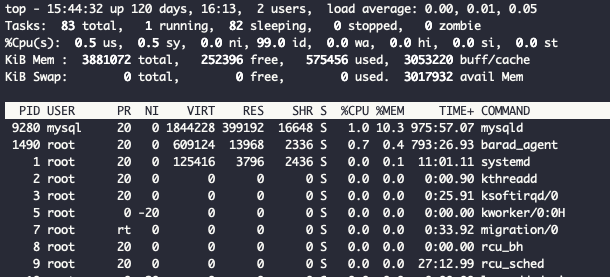
\includegraphics[width=1\textwidth]{linux/top-1.png}
    \caption{top}
\end{figure}


第一行输出任务为UPTIME and LOAD Averages

\begin{lstlisting}[language=cshell]

#   top - 15:52:24 up 120 days, 16:21,  2 users,  load average: 0.14, 0.10, 0.07

\end{lstlisting}

第二行为任务(进程)或者线程信息;进程或者线程的切换可以通过交互命令H。 分为:运行;休眠;停止;僵尸

\begin{lstlisting}[language=cshell]

#   Tasks:  86 total,   1 running,  85 sleeping,   0 stopped,   0 zombie

#   Threads: 149 total,   1 running, 148 sleeping,   0 stopped,   0 zombie

\end{lstlisting}


第三行为CPU状态信息


\begin{lstlisting}[language=cshell]

#   %Cpu(s):  0.7 us,  0.7 sy,  0.0 ni, 98.7 id,  0.0 wa,  0.0 hi,  0.0 si,  0.0 st
#              a   b      c  d 
#   %Cpu(s):  0.3/0.5     1[|

\end{lstlisting}

us, user    : 用户空间占用CPU百分比(time running un-niced user processes)    \par
sy, system  : 内核空间占用CPU百分比(time running kernel processes)  \par
ni, nice    : 用户进程空间内改变过优先级的进程占用CPU百分比(time running niced user processes)   \par
id, idle    : 空闲CPU百分比(time spent in the kernel idle handler)  \par
wa, IO-wait : 等待输入输出的CPU时间百分比(time waiting for I/O completion)       \par
hi : 硬中断(Hardware IRQ)占用CPU的百分比(time spent servicing hardware interrupts)      \par
si : 软中断(Software Interrupts)占用CPU的百分比(time spent servicing software interrupts)      \par
st : hypervisor vm占用的CPU时间的百分比(time stolen from this vm by the hypervisor) \par

在使用交互命令t切换到cpu状态模式时,还会额外显示一行CPU摘要信息,如上面展示第二行

a) 是 us 和 ni 之和 \par
b) 是 sy 百分比 \par
c) 是总和   \par
d) 是可视化图像 \par


内存使用情况

默认情况下,第1行反映物理内存,分类为:\par
total(物理内存总量), free(空闲内存总量), used(使用的物理内存总量) and buff/cache(用作内核缓存的内存量)

第2行反映的主要是虚拟内存,分为以下几类:\par
total(交换区总量), free(闲交换区总量), used(使用的交换区总量) and avail(可用物理内存)

此行的avail 指启动新应用程序时可用的物理内存的估计值不包含swapping。与free命令不同的是,free试图分析易于回收的页面缓存和内存片。

可以通过交互命令E切换单位

\begin{lstlisting}[language=cshell]

# MiB Mem :   3790.1 total,    228.7 free,    568.1 used,   2993.2 buff/cache
# MiB Swap:      0.0 total,      0.0 free,      0.0 used.   2941.0 avail Mem

\end{lstlisting}

在内存模式(使用交互命令m)下,会显示两行简短的简要:

\begin{lstlisting}[language=cshell]

            a    b          c
MiB Mem : 23.2/3790.1   [|||||                         ]
MiB Swap:  0.0/0.0      [                              ]

\end{lstlisting}

a) 使用百分比

b) 总物理内存

c) 图形化展示


\begin{lstlisting}[language=cshell]

PID USER      PR  NI    VIRT    RES    SHR S  %CPU %MEM     TIME+ COMMAND
9280 mysql     20   0 1844228 399192  16648 S   0.7 10.3 990:08.75 mysqld
1490 root      20   0  609124  13968   2336 S   0.3  0.4 803:34.96 barad_agent

\end{lstlisting}

\subsection{列字段含义}

1. \%CPU  -- CPU使用率  \par
\qquad CPU使用时间占比;

2. \%MEM  --  内存使用 (RES)   \par
\nftt{进程当前使用的可用物理内存占比}

3. CGROUPS  --  Control Groups  \par

4. CODE  --  Code Size (KiB) \par
\nftt{可执行代码占用物理内存大小,也称为文本常驻集(Text Resident Set)大小或TRS。}

5. COMMAND  --  命令名/命令行   \par

6. DATA  --  Data + Stack Size (KiB) 数据段 + 栈    \par
\nftt{可执行代码以外的物理内存的大小,也称为数据常驻集大小或DRS。}

7. ENVIRON  --  环境变量   \par

8. Flags  --  Task Flags    \par
\nftt{This column represents the task's current scheduling flags which are expressed in hexadecimal notation and with zeros suppressed.  These flags are officially documented in <linux/sched.h>.}

9. GID  --  有效组ID \par

10. GROUP  --  有效组名 \par

11. NI  --  Nice Value 进程的nice值。nice值越小优先级越高。 0表示不调整优先级。  \par

12. P  --  Last used CPU (SMP)  \par
\nftt{A number representing the last used processor.  In a true SMP environment this will likely change frequently since the kernel intentionally uses weak affinity.  Also, the very act of running top may break this weak affinity and cause  more  processes  to
change CPUs more often (because of the extra demand for cpu time).}

13. PGRP  --  进程组ID  \par

14. PID  --  进程ID \par

15. PPID  --  父进程ID \par

16. PR  --  优先级   \par
可以使用chrt命令查看进程调度

进程调度分为Normal Scheduling和Real-time Scheduling

Normal Scheduling: SCHED\_OTHER      SCHED\_IDLE   SCHED\_BATCH

Real-time Scheduling: SCHE\_FIFO     SCHED\_RR

Priority value: [1,99] 值越低优先级越高

Normal Scheduling priority默认值为0

SCHED\_OTHER: 对应time-sharing policy (RR)

PR值和NICE仅对Normal Scheduling进程有效;
PR = 20 + NICE(友好值[-20,19]) = [0,39] PR值越高优先级越低

SCHED\_FIFO和SCHED\_RR  real-time process/thread

priority = [1,99]
PR = -1 - priority = [-100, -2]

\nftt{进程调度优先级。如果在字段中看到rt,则说明该线程是Real-time Scheduling。}

17. RES  --  进程占用内存大小 (KiB) \par
\nftt{进程使用的未被swap物理内存大小(The non-swapped physical memory a task is using.)}

18. RUID  --  真实用户id \par

19. RUSER  --  真实用户名 \par

20. S  --  进程状态(Process Status) \par
\begin{itemize}
    \item \nftt{ D = 不可中断睡眠状态(uninterruptible sleep) }
    \item \nftt{ R = 运行状态(running)   }
    \item \nftt{ S = 睡眠状态(sleeping) }
    \item \nftt{ T = stopped by job control signal  }
    \item \nftt{ t = stopped by debugger during trace   }
    \item \nftt{ Z = 僵尸状态(zombie)   }
\end{itemize}

\nftt{D状态一般为等待IO,例如磁盘IO、网络IO等。}

21. SHR  --  共享内存大小(Shared Memory Size) (KiB)   \par
\nftt{进程可用的共享内存大小,通常不是所有的都驻留。它只能反应可能与其他进程共享的内存。}

22. SID  -- 会话ID \par

23. SUID  --  Saved User Id \par

24. SUPGIDS  --  附属组ID    \par

25. SUPGRPS  --  附属组名  \par

26. SUSER  --  Saved User Name  \par

27. SWAP  --  Swapped Size (KiB)  线程地址空间的非驻留部分  \par

28. TGID  --  线程组ID(Thread Group Id) \par
\nftt{任务所属的线程组的ID。它是线程组领导的PID。在内核术语中,它表示那些共享mm\_struct的任务。}

29. TIME  --  CPU Time  \par
\nftt{线程启动后使用的总CPU时间。当启用累积模式时,将列出每个进程以及其死去的字进程所使用的CPU时间。可以使用交互命令S来切换累积模式。}

30. TIME+  --  CPU Time, hundredths \par
\nftt{与TIME相同,但通过百分之一秒反映出更细的粒度。}

31. TPGID  --  Tty Process Group Id \par

32. TTY  --  Controlling Tty    \par

33. UID  --  用户ID;进程所有者的真实用户ID   \par

34. USED  --  Memory in Use (KiB)   \par
\nftt{此字段表示线程使用的非swapped物理内存(RES)及其地址空间的非驻留部分(SWAP)。}

35. USER  --  用户名;进程所有者的真实用户名  \par

36. VIRT  --  虚拟内存大小(Virtual Memory Size)(KiB) \par
\nftt{进程使用的虚拟内存大小。包括代码,数据以及共享库以及已换出的页和已映射但未使用的页。}

37. WCHAN  --  Sleeping in Function \par
\nftt{若该进程在睡眠,则显示睡眠中的系统函数名。}

38. nDRT  --  脏页数量(Dirty Pages Count) \par
\nftt{The number of pages that have been modified since they were last written to auxiliary storage.  Dirty pages must be written to auxiliary storage before the corresponding physical memory location can be used for some other virtual page.}

39. nMaj  --  Major Page Fault Count    \par
\nftt{The number of major page faults that have occurred for a task.  A page fault occurs when a process attempts to read from or write to a virtual page that is not currently present in its address space.  A major page fault is when auxiliary  storage  access
is involved in making that page available.}

40. nMin  --  Minor Page Fault count    \par
\nftt{The number of minor page faults that have occurred for a task.  A page fault occurs when a process attempts to read from or write to a virtual page that is not currently present in its address space.  A minor page fault does not involve auxiliary storage
access in making that page available.}

41. nTH  --  线程数量  \par

42. nsIPC  --  IPC namespace    \par
\nftt{The Inode of the namespace used to isolate interprocess communication (IPC) resources such as System V IPC objects and POSIX message queues.}

43. nsMNT  --  MNT namespace    \par
\nftt{The Inode of the namespace used to isolate filesystem mount points thus offering different views of the filesystem hierarchy.}

44. nsNET  --  NET namespace    \par
\nftt{The Inode of the namespace used to isolate resources such as network devices, IP addresses, IP routing, port numbers, etc.}

45. nsPID  --  PID namespace    \par
\nftt{The Inode of the namespace used to isolate process ID numbers meaning they need not remain unique.  Thus, each such namespace could have its own `init' (PID \#1) to manage various initialization tasks and reap orphaned child processes.}

46. nsUSER  --  USER namespace  \par
\nftt{The Inode of the namespace used to isolate the user and group ID numbers.  Thus, a process could have a normal unprivileged user ID outside a user namespace while having a user ID of 0, with full root privileges, inside that namespace.}

47. nsUTS  --  UTS namespace    \par
\nftt{The Inode of the namespace used to isolate hostname and NIS domain name.  UTS simply means "UNIX Time-sharing System".}

48. vMj  --  Major Page Fault Count Delta   \par
\nftt{The number of major page faults that have occurred since the last update (see nMaj).}

49. vMn  --  Minor Page Fault Count Delta   \par
\nftt{The number of minor page faults that have occurred since the last update (see nMin).}


\subsection{示例}

\begin{figure}[H]
    \centering
    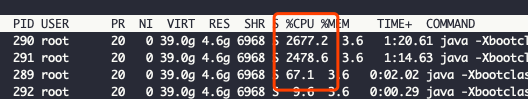
\includegraphics[width=1\textwidth]{linux/top_cpu_over_100.png}
    \caption{top cpu利用率超过100\%}
\end{figure}

\subsubsection{如上图所示:CPU使用率超过100\%}

这里CPU使用率是所有CPU的总和。即你的CPU是多核处理器。可以使用交互式命令1来查看所有CPU的使用情况。









